\documentclass[9pt, spanish]{beamer}\usepackage[]{graphicx}\usepackage[]{color}
%% maxwidth is the original width if it is less than linewidth
%% otherwise use linewidth (to make sure the graphics do not exceed the margin)
\makeatletter
\def\maxwidth{ %
  \ifdim\Gin@nat@width>\linewidth
    \linewidth
  \else
    \Gin@nat@width
  \fi
}
\makeatother

\definecolor{fgcolor}{rgb}{0.345, 0.345, 0.345}
\newcommand{\hlnum}[1]{\textcolor[rgb]{0.686,0.059,0.569}{#1}}%
\newcommand{\hlstr}[1]{\textcolor[rgb]{0.192,0.494,0.8}{#1}}%
\newcommand{\hlcom}[1]{\textcolor[rgb]{0.678,0.584,0.686}{\textit{#1}}}%
\newcommand{\hlopt}[1]{\textcolor[rgb]{0,0,0}{#1}}%
\newcommand{\hlstd}[1]{\textcolor[rgb]{0.345,0.345,0.345}{#1}}%
\newcommand{\hlkwa}[1]{\textcolor[rgb]{0.161,0.373,0.58}{\textbf{#1}}}%
\newcommand{\hlkwb}[1]{\textcolor[rgb]{0.69,0.353,0.396}{#1}}%
\newcommand{\hlkwc}[1]{\textcolor[rgb]{0.333,0.667,0.333}{#1}}%
\newcommand{\hlkwd}[1]{\textcolor[rgb]{0.737,0.353,0.396}{\textbf{#1}}}%
\let\hlipl\hlkwb

\usepackage{framed}
\makeatletter
\newenvironment{kframe}{%
 \def\at@end@of@kframe{}%
 \ifinner\ifhmode%
  \def\at@end@of@kframe{\end{minipage}}%
  \begin{minipage}{\columnwidth}%
 \fi\fi%
 \def\FrameCommand##1{\hskip\@totalleftmargin \hskip-\fboxsep
 \colorbox{shadecolor}{##1}\hskip-\fboxsep
     % There is no \\@totalrightmargin, so:
     \hskip-\linewidth \hskip-\@totalleftmargin \hskip\columnwidth}%
 \MakeFramed {\advance\hsize-\width
   \@totalleftmargin\z@ \linewidth\hsize
   \@setminipage}}%
 {\par\unskip\endMakeFramed%
 \at@end@of@kframe}
\makeatother

\definecolor{shadecolor}{rgb}{.97, .97, .97}
\definecolor{messagecolor}{rgb}{0, 0, 0}
\definecolor{warningcolor}{rgb}{1, 0, 1}
\definecolor{errorcolor}{rgb}{1, 0, 0}
\newenvironment{knitrout}{}{} % an empty environment to be redefined in TeX

\usepackage{alltt}
%\usepackage[dvips]{graphicx}
\usepackage[spanish]{babel}
\selectlanguage{spanish}
\usepackage[utf8]{inputenc}
\usepackage{mathptmx}
\usepackage{verbatim}
\usepackage{fancyvrb}
\usepackage{lipsum}
\usepackage{natbib}
\usepackage{verbatimbox}
\usepackage{beamerthemesplit}
\useinnertheme{circles,rounded}

% \usepackage{etoolbox}
% \patchcmd{\thebibliography}{\section*{\refname}}{}{}{}


\definecolor{uofsgreen}{RGB}{136,57,138}
\usecolortheme[named=uofsgreen]{structure}
%\usetheme[height=7mm]{Rochester} 
%\useoutertheme{smoothtree}
%\usecolortheme{structure}
%\usetheme{Darmstadt}
%\usefonttheme[onlylarge]{structurebold}
%\setbeamerfont{frametitle}{size=\normalsize,series=\bfseries}
%\setbeamertemplate{navigation symbols}{}

\author{Instituto de Estadística (IESTA)\\
Natalia da Silva\\
@pacocuak
}

\title{Importancia de la Visualizaci\'on Estad\'istica}
\IfFileExists{upquote.sty}{\usepackage{upquote}}{}
\begin{document}
 \frame{\titlepage}

\begin{frame}
\frametitle{De que voy a hablar}
\begin{itemize}
\item Porqu\'e y para qu\'e visualizar

\item Visualizaci\'on estad\'istica

\item Ideas para una visualizaci\'on efectiva

\end{itemize}
\end{frame}

\begin{frame}
\frametitle{Importancia de la Visualizaci\'on }

"The greatest value of a picture is when it forces us to notice what we never expected to see."   \cite{tukey77}

\vspace{1cm}

% J. W. Tukey (1977)

% una parte importante de la practiac estadistica es la comunicacion grafica de datos y modelos y esta es una parte importante de la theoria estadistica
\end{frame}


\begin{frame}
\frametitle{Pocos se escapan a este pensamiento}

\begin{itemize}
\item Los c\'alculos num\'ericos son exactos pero los gr\'aficos son toscos o aproximados

\item Para cada tipo de datos estad\'isticos hay un conjunto de c\'alculos que constituyen un an\'alisis estad\'istico correcto

\item Hacer c\'alculos intrincados es virtuoso mientras que mirar los datos es hacer trampa, \cite{anscombe}

\end{itemize}

\end{frame}

\begin{frame}
\frametitle{Visualizaci\'on Estad\'istica}
La visualizaci\'on juega un rol importante en todas las etapas del an\'alisis estad\'istico.
\begin{itemize}
\item \textbf{Exploraci\'on}: Encontrar patrones generales y espec\'ificos en los datos. 
\item \textbf{Modelado}: Chequear supuestos sobre los datos antes de modelar.
Se puede hacer inferencia gr\'afica (nueva linea).
\item \textbf{Diagn\'ostico}: Visualizar el modelo en el espacio de los datos \'o los datos en el espacio del modelo.
\end{itemize}
\end{frame}

\begin{frame}
\frametitle{¿Cu\'al es la relaci\'on entre x e y?}
\begin{center}
\begin{tabular}{ c | c  }
  \hline			
  x&	y\\ \hline
1.972&	1.236\\
1.112&	1.994\\
0	&1.009\\
0.665&	1.942\\
0.235&	0.356\\
0.247&	1.658\\
1.275&	1.961\\
0.702&	0.045\\
1.76&	0.35\\
1.691&	0.277\\
1.628&	1.778\\
1.957&	1.29\\
  \hline  
\end{tabular}
\end{center}
% la tabla y el plot contienene exactamente la misma info
%con la figura es inmediatamente ovbia la relacion porque lo que esta 
%jugando es la pre-attentive proceso que es la acumulacion inconciente de informacion del ambiente
%demoramos milesimas de segundo para ver que es un circulo
\end{frame}

\begin{frame}
\frametitle{¿Porqu\'e usamos visualizaci\'on?}
\begin{center}
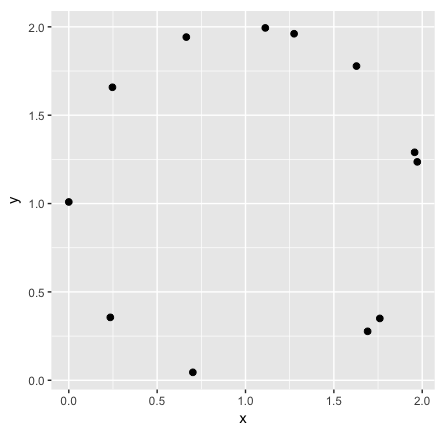
\includegraphics[width=5cm]{Circulo}
\end{center}
\begin{center}
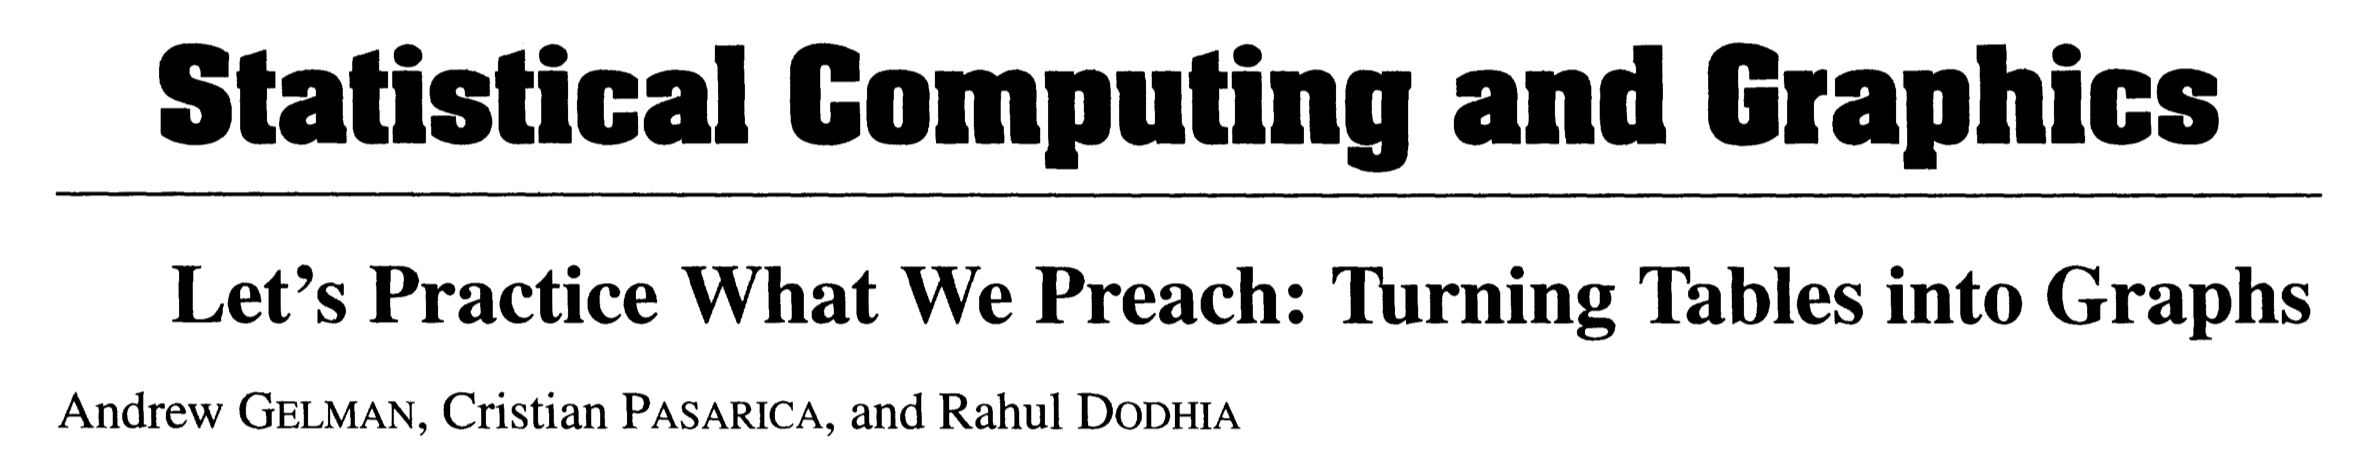
\includegraphics[width=9cm]{gelman}
\end{center}
\end{frame}


\begin{frame}
\frametitle{¿Porqu\'e usamos visualizaci\'on?}

\begin{columns}
\begin{column}{4cm}
\begin{itemize}
\item Los g\'aficos proveen m\'as informac\'on que los res\'umenes num\'ericos
\item Anscombe’s quartet \cite{anscombe}
\begin{tabular}{l}
 $n = 11$ \\
$\bar x= 9.0$ \\
 $\bar y = 7.5$ \\
 $\hat \beta_1= 0.5$ \\
$ y = 3 + 0.5 x$ \\
 $R^2 = 0.667$ \\
$....$
\end{tabular}
% \item Sum of squares of x - 110.0
% \item Regression sum of squares = 27.50 (1 d.f.) 
% \item Residual sum of squares of y = 13.75 (9 d.f.)
% \item Estimated standard error of bi = 0.118
% \item Multiple R2 = 0.667

\end{itemize}

\end{column}
\begin{column}{8cm}

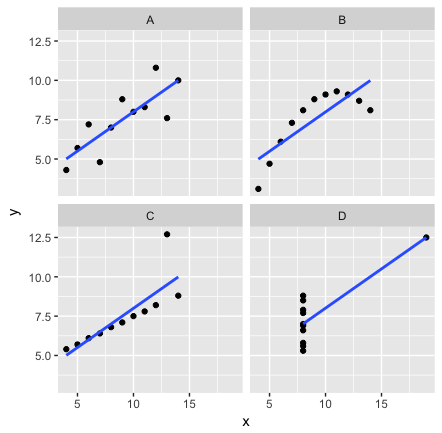
\includegraphics[width=8cm]{Quartet} 
\end{column}
\end{columns}
\end{frame}

% \begin{frame}
% \frametitle{¿Cu\'al es la media?}
% \begin{center}
% \includegraphics[width=8cm]{img1} 
% \end{center}
% \end{frame}


% 
% \begin{frame}
% \frametitle{¿Cu\'al es la media?}
% \begin{center}
% \includegraphics[width=8cm]{imag2} 
% \end{center}
% \end{frame}
% 
% 
\begin{frame}
\frametitle{¿Porqu\'e usamos visualizaci\'on?}

\begin{center}
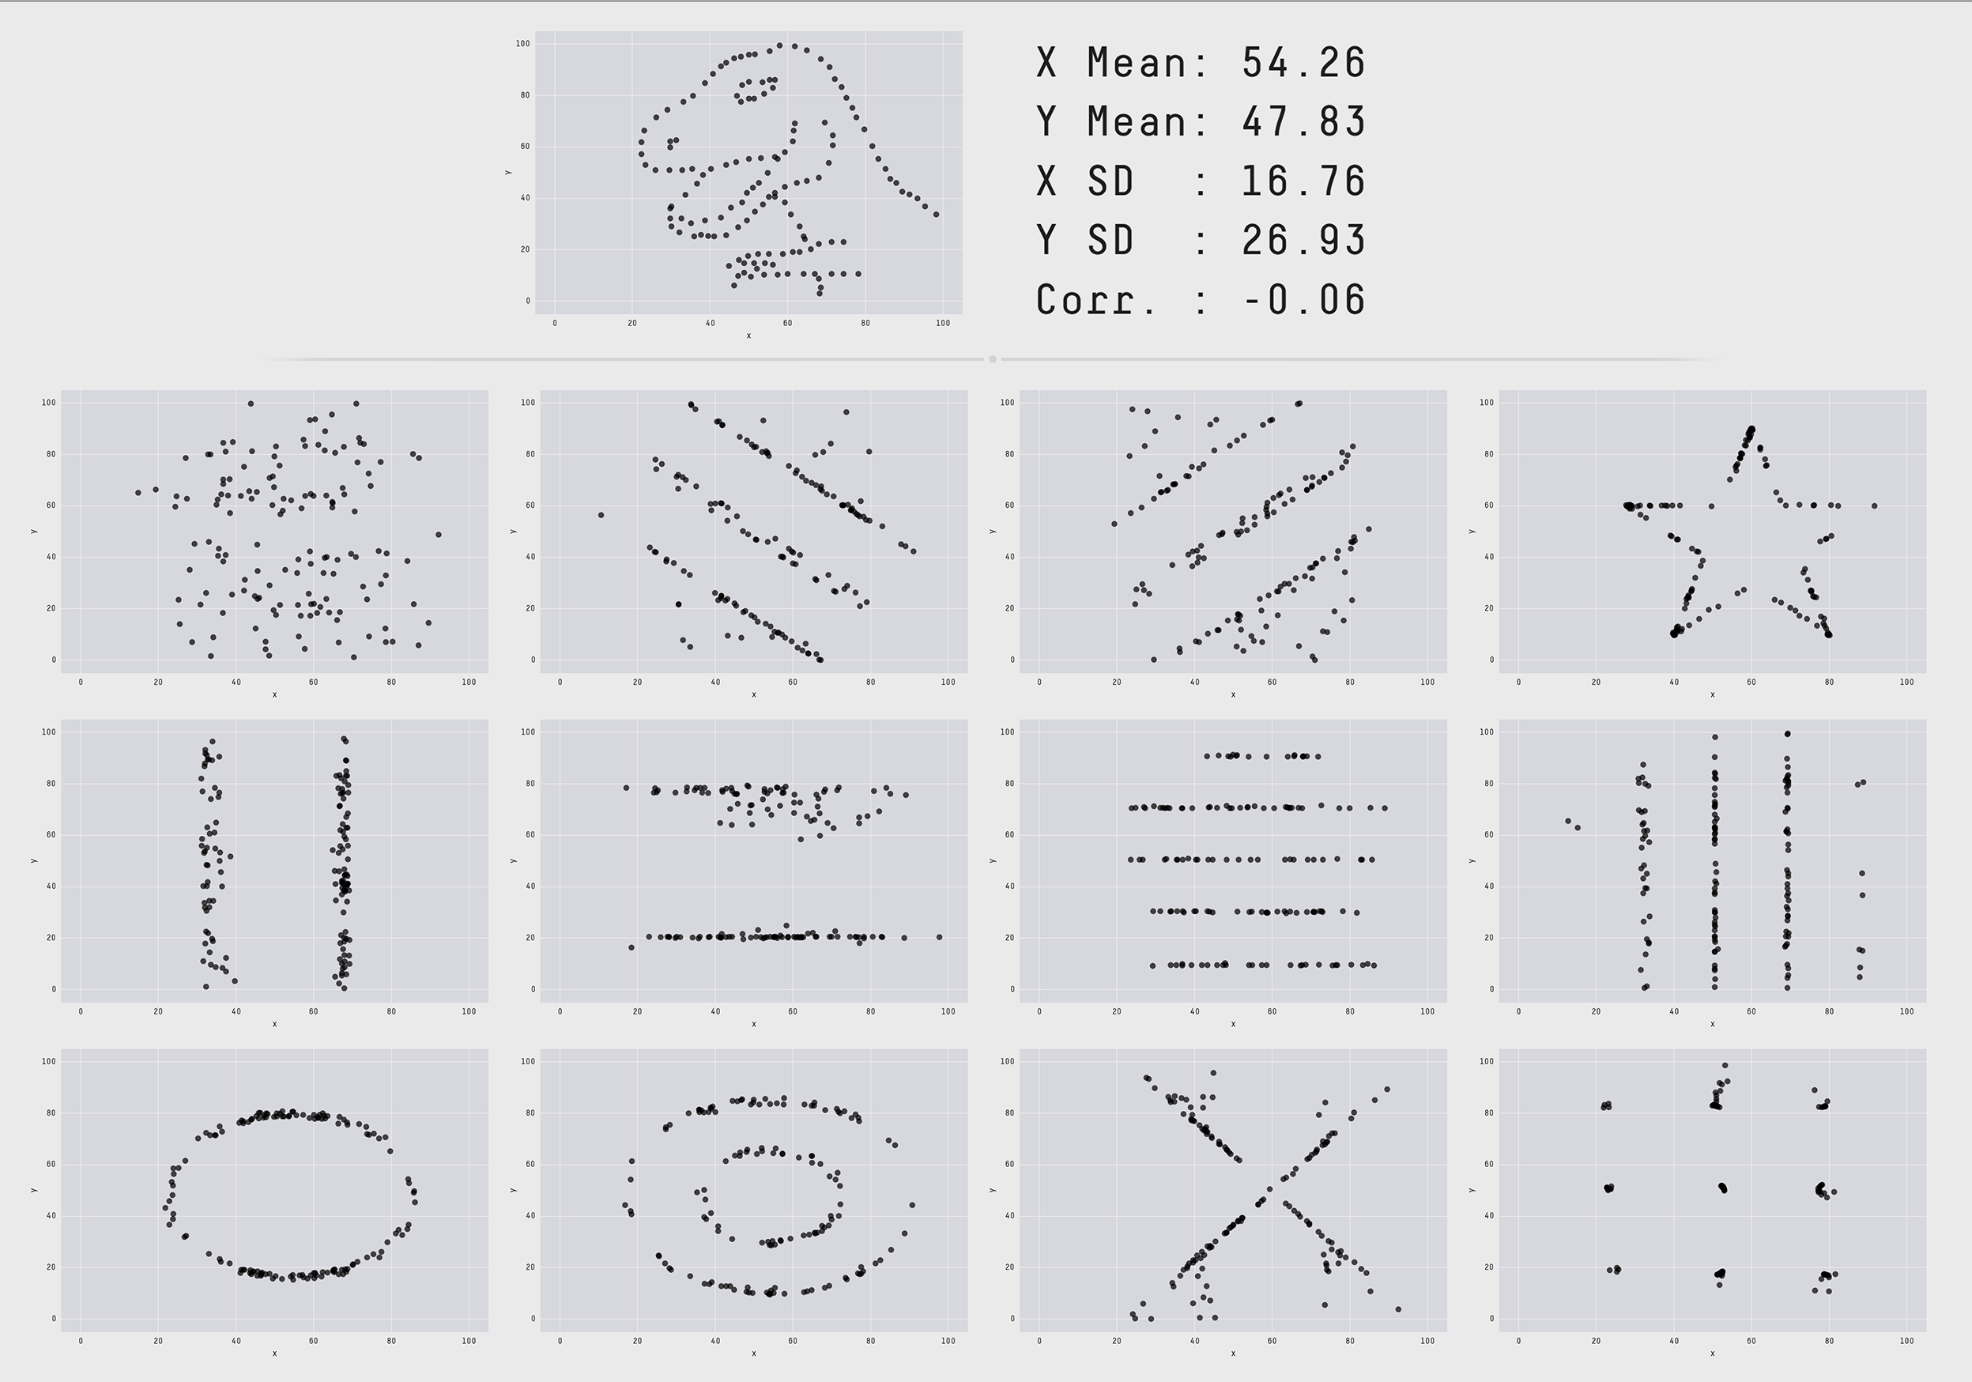
\includegraphics[width=8cm]{dino}
\end{center}
https://github.com/stephlocke/datasauRus

Los res\'umenes estad\'isticos pueden ser los mismos pero las distribuciones muy diferentes
\end{frame}


\begin{frame}
\begin{itemize}
\frametitle{Visualizaciones efectivas?}
\item No todas las visualizaciones son igualmente efectivas
\item Hay diferentes criterios para evaluar gr\'aficos (Cleveland, Tufte, Car, Wainer, etc  )
%usando Cleveland view
\item Basado en el estudio de la percepci\'on gr\'afica de Cleveland \citep{cleveland},
las mejores visualizaciones son aquellas que requieren el uso de la visi\'on "pre-attentive" (instantaneo, sin aparente esfuerzo visual)

\end{itemize}
\end{frame}

\begin{frame}
\frametitle{Cleveland, Percepci\'on gr\'afica}
\begin{center}
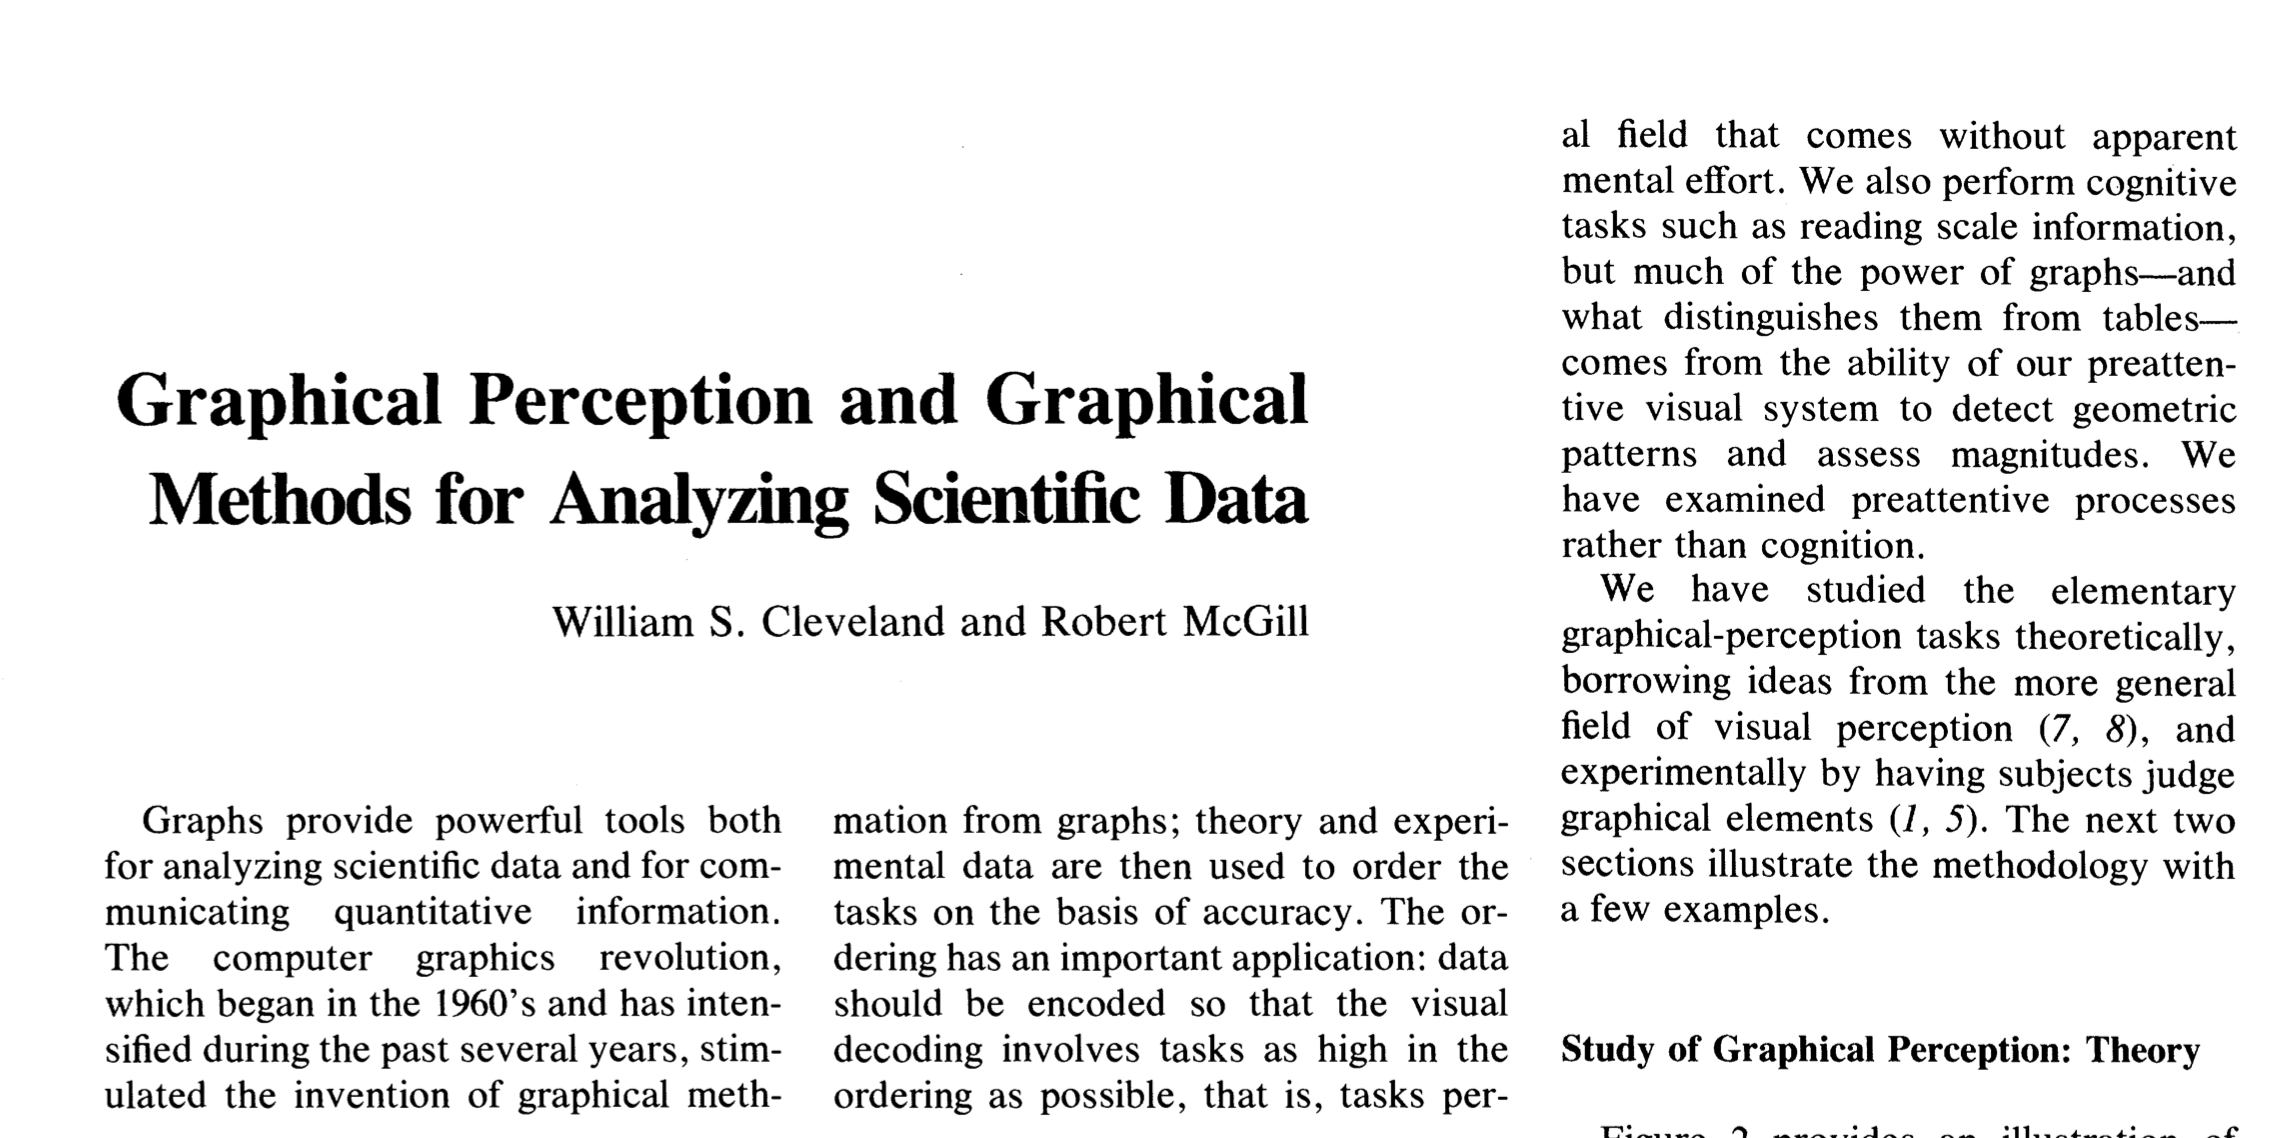
\includegraphics[width=8cm]{cleveland}
\end{center}
\end{frame}

\begin{frame}
\frametitle{¿C\'omo decodificamos un gr\'afico? }


\begin{itemize}
\item Cuando miramos un gr\'afico la informaci\'on es visualmente decodificada por el sistema visual de la persona
\item Un m\'etodo gr\'afico es efectivo solamente si la decodificaci\'on lo es

\item Buenas visualizaciones son las que optimizan el sistema visual humano

\item Si esto es verdad tendr\'iamos que saber c\'omo el sistema humano decodifica un gr\'afico
\end{itemize}

% Tres operaciones visuales de la percepci\'on de patrones por Cleveland:
% \begin{itemize}
% \item \textbf{Deteci\'on:} reconocimiento visual de un objeto geométrico codificado en un valor f\'isico
% \item \textbf{Ensamblado:} es el agrupado de elementos gr\'aficos detectados
% \item \textbf{Estimaci\'on:} es la actividad visual de los valores relativos de 2 o mas valores cuantitativos
% %(mayor menor distinto ratios etc)
% \end{itemize}
\end{frame}



\begin{frame}
\frametitle{Comparar variables cuantitativas}
Cleveland ordena la dificultad de los elementos 
gr\'aficos basado en la percepci\'on para estimar variables cuantitativas

\begin{enumerate}
\item Posici\'on a lo largo de una escala com\'un
\item Posici\'on en escals no alineadas pero ide\'enticas
\item Longitud
\item \'Angulo \'o pendiente
\item \'Area
\item Vol\'umen, densidad \'o saturaci\'on del color
\item Tono del color
\end{enumerate}
\end{frame}

\begin{frame}
\frametitle{¿C\'omo uso esto?}
\begin{itemize}
\item Cu\'al es la comparaci\'on m\'as importante que quiero hacer cuando tengo variables cuantitativas
\item Tenemos que codificar eso que quiero comparar usando los elementos gr\'aficos en la tabla en orden ( 1. posiciones en la misma escala )
\end{itemize}
\end{frame}


\begin{frame}
\frametitle{Comparar millas por gal\'on (mpg)}
\begin{columns}
\begin{column}{4cm}
7) Color
\includegraphics[width=4cm]{color}
\end{column}
\begin{column}{4cm}
3) Longitud
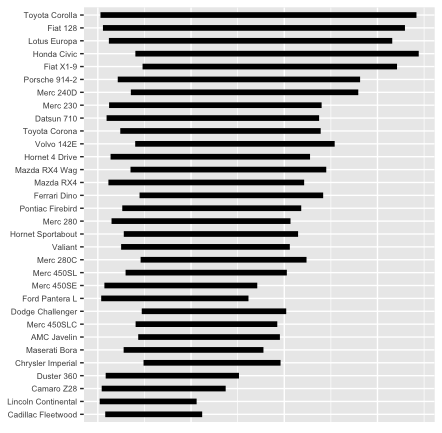
\includegraphics[width=4cm]{lenght}
\end{column}
\begin{column}{4cm}
1) Posici\'on, escala com\'un
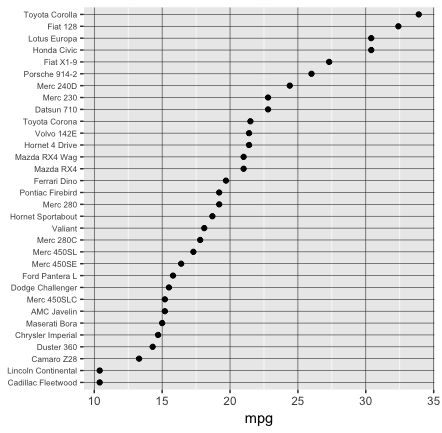
\includegraphics[width=4cm]{Scaled}
\end{column}
\end{columns}
\end{frame}
% \begin{frame}
% \frametitle{Reglas de Tufte}
% \begin{enumerate}
% \item Muestra los datos
% \item Inducir al usuario a pensar en los datos
% \item Evit\'a distorcionar lo que los datos tienen para decir
% \item
% item
% \end{enumerate}
% \end{frame}

\begin{frame}
\frametitle{\'Angulo \'o pendiente}
\begin{itemize}
\item Gr\'aficos de torta son siempre un error!!!

\item Pero ahora sabemos porqu\'e

\item Porque decodificar variables cuantitativas usando \'anglulos es m\'as dif\'icil que con otros elementos gr\'aficos 

\item Siempre es preferible un gr\'afico de barras a uno de torta

\end{itemize}
\end{frame}

\begin{frame}
\frametitle{Visualizaci\'on para comunicar adecuadamente}

\begin{columns}
\begin{column}{6cm}
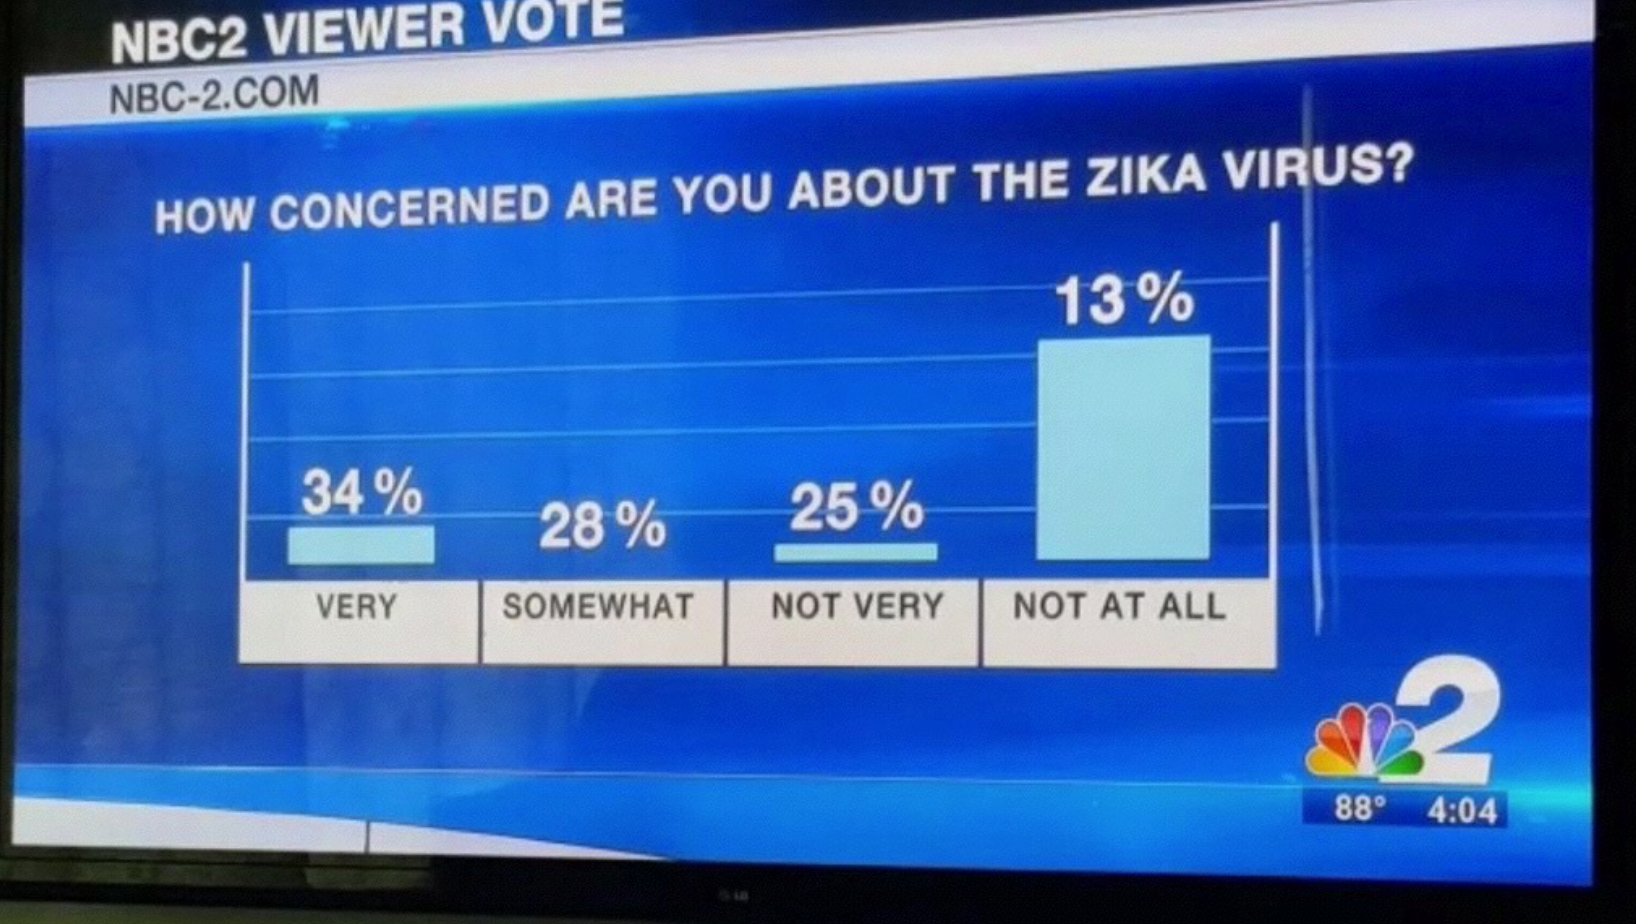
\includegraphics[width=5cm]{ej1}
\end{column}

\begin{column}{6cm}
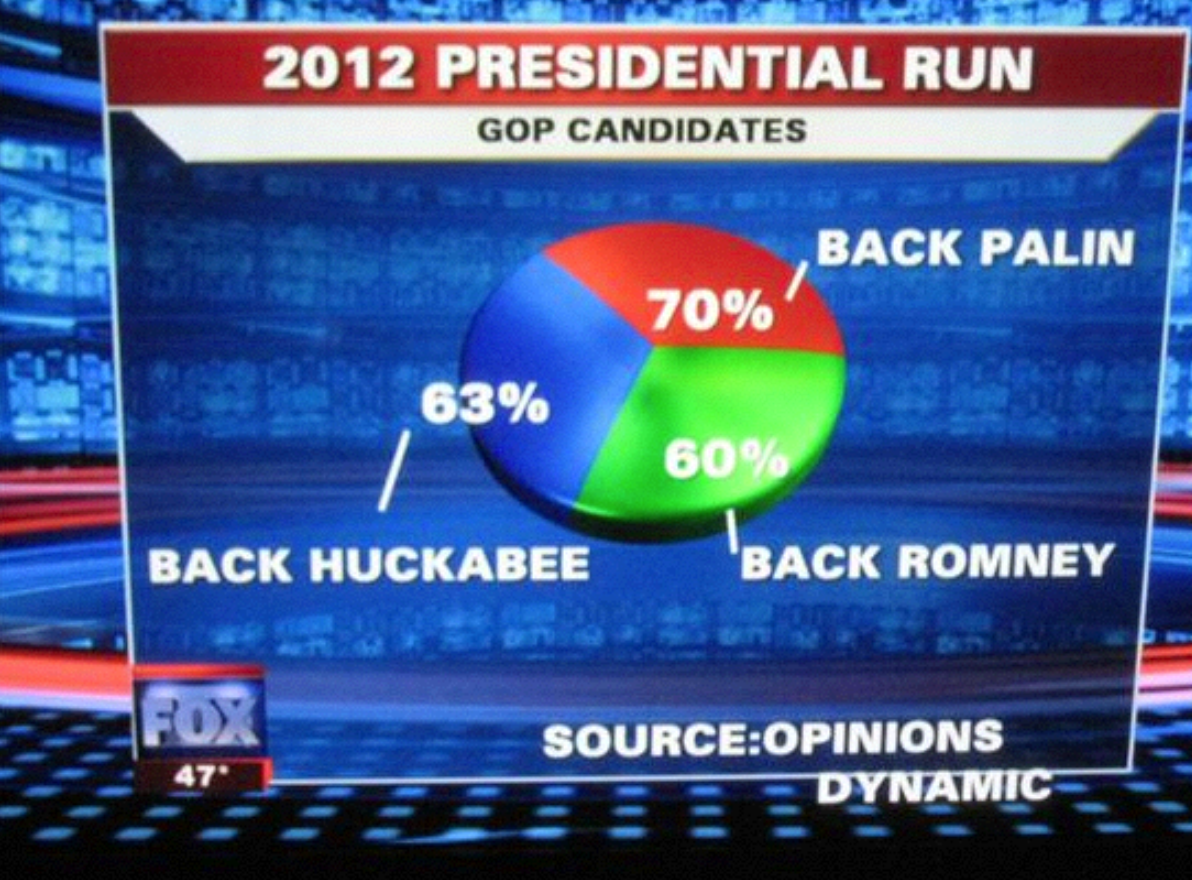
\includegraphics[width=5cm]{ej2}
\end{column}
\end{columns}
\end{frame}

\begin{frame}
\frametitle{Herramientas para Visualizar}
\begin{itemize}
\item ggplot2 \citep{wickham2016ggplot2} es un paquete para producir gráficos estadísticos o de datos que a diferencia tiene una teoría que lo sustenta basada en Grammar of Graphics \citep{wilkinson2006grammar}


\item Aprender en base a una grámatica gráfica te permite graficar cosas que sabés pero además crear nuevas y tal vez mejores gráficos para visualizar tus datos.
\end{itemize}
\end{frame}

\begin{frame}
\frametitle{Comentarios Finales}
\begin{itemize}
\item Visualizaci\'on es importante en todas las etapas del an\'alisis esta\'istico
\item Hacer visualizaci\'on efic\'az permite comunicar los resultados de forma sencilla
\item Para estimar cantidades el elemento gr\'afico m\'as efic\'az es la posici\'on a lo largo de una escala com\'un
\item Hacer visualizaci\'on efic\'az no es trivial, requiere conocimiento y trabajo
\item Herramienta basada en gr\'amatica gr\'afica en R para producir gr\'aficos de alta calidad, ggplot2
\end{itemize}
\end{frame}





\begin{frame}{Bibliograf\'ia}
\renewcommand\refname{\vskip -1cm}
\bibliographystyle{asa}
%\bibliographystyle{plain}
\bibliography{bibliophd}
\end{frame}
\end{document}
